% 1977 年黑龙江卷第 5 题：△ABC 内接于圆，∠A 的平分线 AE 交 BC 于 D、交外接圆于 E（按源卷布局）
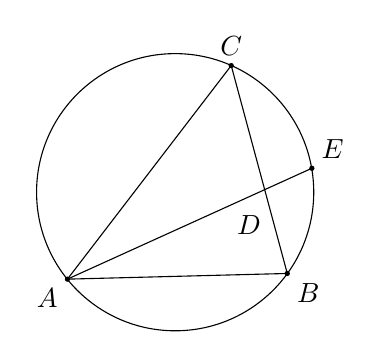
\begin{tikzpicture}[scale=0.8]
  \draw (0,0) circle (2.2);
  \coordinate (A) at (-1.71,-1.38);
  \coordinate (B) at (1.78,-1.29);
  \coordinate (C) at (0.89,2.01);
  \coordinate (E) at (2.17,0.38);
  \coordinate (D) at (1.42,0.04);
  \draw (A) -- (B) -- (C) -- cycle;
  \draw (A) -- (E);
  \fill (A) circle (1.2pt) node[below left] {$A$};
  \fill (B) circle (1.2pt) node[below right] {$B$};
  \fill (C) circle (1.2pt) node[above] {$C$};
  \fill (E) circle (1.2pt) node[above right] {$E$};
  \node at (1.17,-0.52) {$D$};
\end{tikzpicture}
